\section{Github}
Link for the every exercises in Lab 1: 

\section{Exercise and Report}
\subsection{Exercise 1}
From the simulation on Proteus, one more LED is connected to pin \textbf{PA6} of the STM32 (negative pin of the LED is connected to PA6). The component suggested in this exercise is \textbf{LED-YELLOW}, which can be found from the device list.\\

In this exercise, the status of two LEDs are switched every 2 seconds, as demonstrated in the figure bellow.

\begin{figure}[!htp]
    \centering
    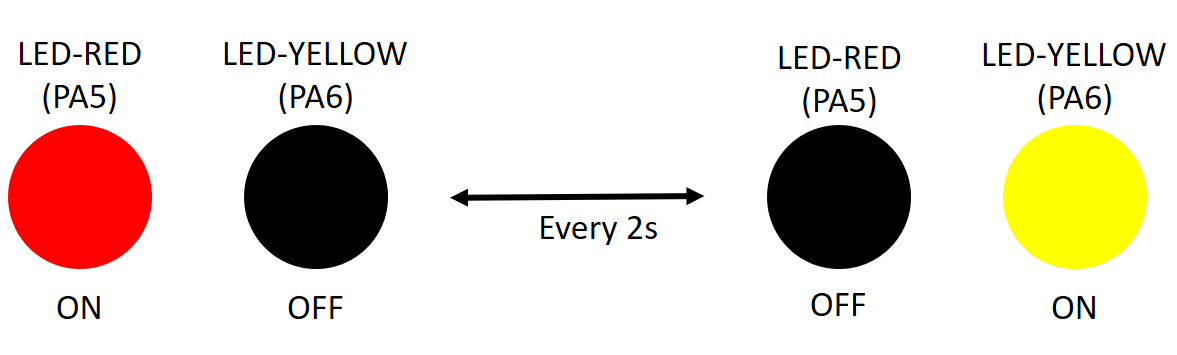
\includegraphics[width=5in]{pictures/bai_1/pic1.PNG}
    \caption{\textit{State transitions for 2 LEDs}}
    \label{bai1_pic1}
\end{figure}

\textbf{Report 1: }Depict the schematic from Proteus simulation in this report. The caption of the figure is a downloadable link to the Proteus project file (e.g. a github link).\\

\begin{figure}[H]
    \centering
    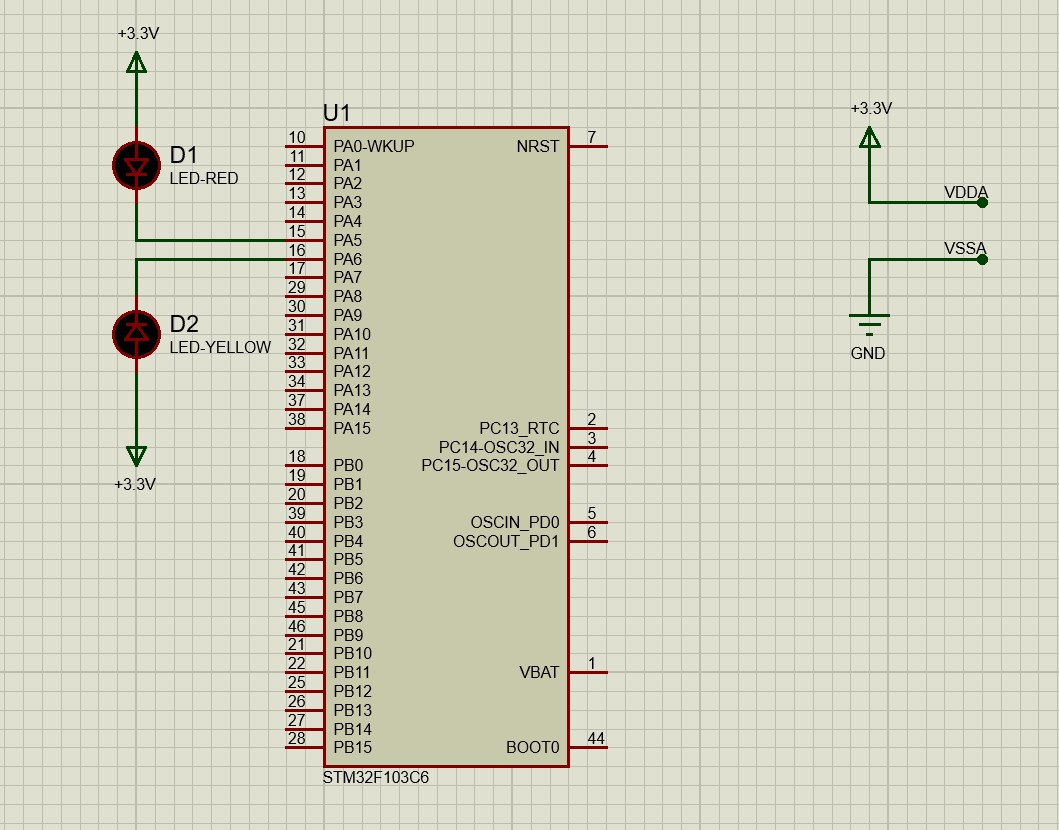
\includegraphics[width=0.6\linewidth]{pictures/schematic_ex01.jpg}
    \caption{\href{https://github.com/Lmonk555/lab01_micro_process_control/tree/563bcd9357e134c12eeb4b0b6b0bf3eb79c213f7/Proteus8/ex_01}{\textit{Proteus schematic for 2 LEDs}}}
    \label{schematic_ex01}
\end{figure}

\textbf{Report 2: } Present the source code in the infinite loop while of your project. If a user-defined functions is used, it is required to present in this part. A brief description can be added for this function (e.g. using comments). A template to present your source code is presented bellow.\\

\begin{lstlisting}[language=c,caption={Exercise 01 source code in while loop},label={lst:ex01}]
    while (1)
    {
        HAL_GPIO_WritePin(LED_RED_GPIO_Port, LED_RED_Pin, GPIO_PIN_RESET);
        HAL_GPIO_WritePin(LED_YELLOW_GPIO_Port, LED_YELLOW_Pin, GPIO_PIN_SET);
        HAL_Delay(2000);

        HAL_GPIO_WritePin(LED_RED_GPIO_Port, LED_RED_Pin, GPIO_PIN_SET);
        HAL_GPIO_WritePin(LED_YELLOW_GPIO_Port, LED_YELLOW_Pin, GPIO_PIN_RESET);
        HAL_Delay(2000);
    }
\end{lstlisting}





\subsection{Exercise 2}
Extend the first exercise to simulate the behavior of a traffic light. A third LED, named \textbf{LED-GREEN} is added to the system, which is connected to \textbf{PA7}. A cycle in this traffic light is 5 seconds for the RED, 2 seconds for the YELLOW and 3 seconds for the GREEN. The LED-GREEN is also controlled by its negative pin.\\

Similarly, the report in this exercise includes the schematic of your circuit and a your source code in the while loop.

\textbf{Report 1: } Present the schematic.\\

\begin{figure}[H]
    \centering
    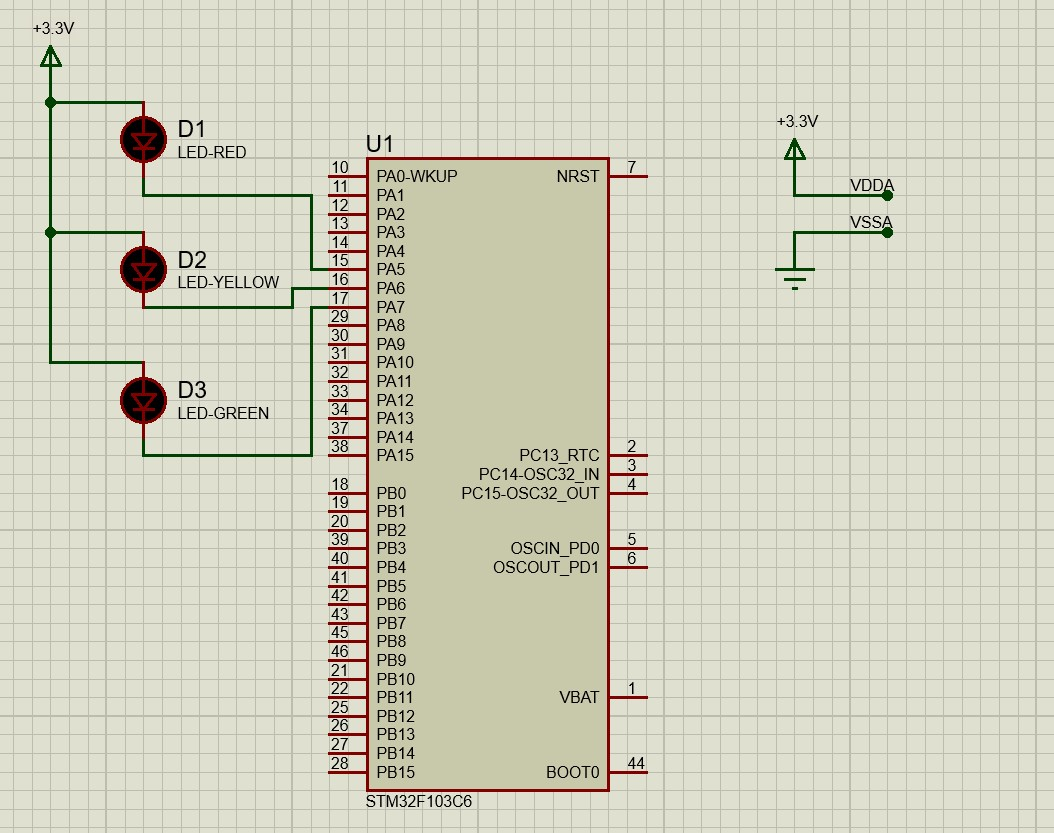
\includegraphics[width=0.8\linewidth]{pictures/schematic_ex02.jpg}
    \caption{\href{https://github.com/Lmonk555/lab01_micro_process_control/tree/99d677862944e732e2b59265c2fbaf87cf88510d/Proteus8/ex_02}{\textit{Proteus schematic for 3 LEDs}}}
    \label{schematic_ex02}
\end{figure}

\textbf{Report 2: } Present the source code in while.\\

\begin{lstlisting}[language=c,caption={Exercise 02 source code in while loop},label={lst:ex02}]
    while (1)
    {
        HAL_GPIO_WritePin(LED_RED_GPIO_Port, LED_RED_Pin, GPIO_PIN_RESET);
        HAL_GPIO_WritePin(LED_YELLOW_GPIO_Port, LED_YELLOW_Pin, GPIO_PIN_SET);
        HAL_GPIO_WritePin(LED_GREEN_GPIO_Port, LED_GREEN_Pin, GPIO_PIN_SET);
        HAL_Delay(5000);

        HAL_GPIO_WritePin(LED_RED_GPIO_Port, LED_RED_Pin, GPIO_PIN_SET);
        HAL_GPIO_WritePin(LED_YELLOW_GPIO_Port, LED_YELLOW_Pin, GPIO_PIN_SET);
        HAL_GPIO_WritePin(LED_GREEN_GPIO_Port, LED_GREEN_Pin, GPIO_PIN_RESET);
        HAL_Delay(3000);

        HAL_GPIO_WritePin(LED_RED_GPIO_Port, LED_RED_Pin, GPIO_PIN_SET);
        HAL_GPIO_WritePin(LED_YELLOW_GPIO_Port, LED_YELLOW_Pin, GPIO_PIN_RESET);
        HAL_GPIO_WritePin(LED_GREEN_GPIO_Port, LED_GREEN_Pin, GPIO_PIN_SET);
        HAL_Delay(2000);
    }
\end{lstlisting}





\subsection{Exercise 3}
Extend to the 4-way traffic light. Arrange 12 LEDs in a nice shape to simulate the behaviors of a traffic light. A reference design can be found in the figure bellow.

\begin{figure}[!htp]
    \centering
    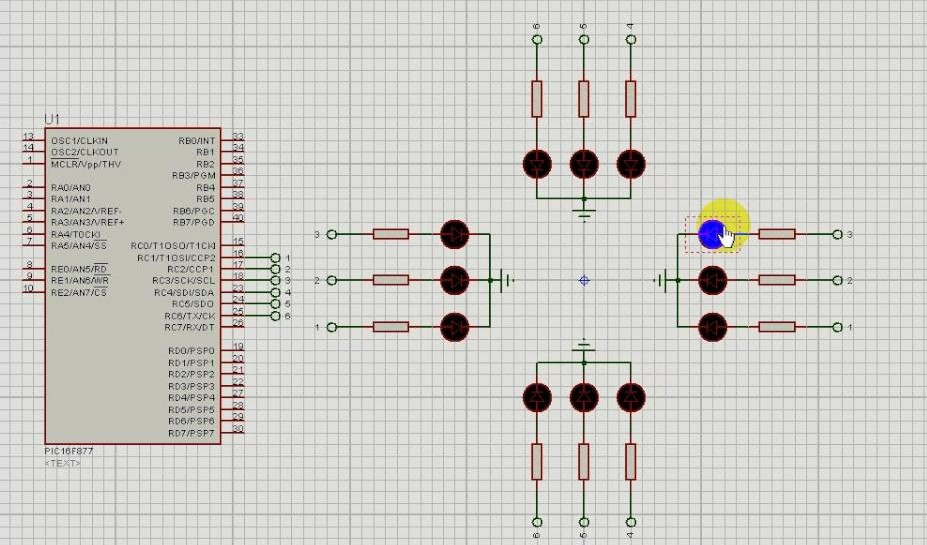
\includegraphics[width=0.8\linewidth]{pictures/bai_1/pic2.jpg}
    \caption{\textit{Reference design for a 4 way traffic light}}
    \label{bai1_pic2}
\end{figure}

\textbf{Report: }

\begin{figure}[H]
    \centering
    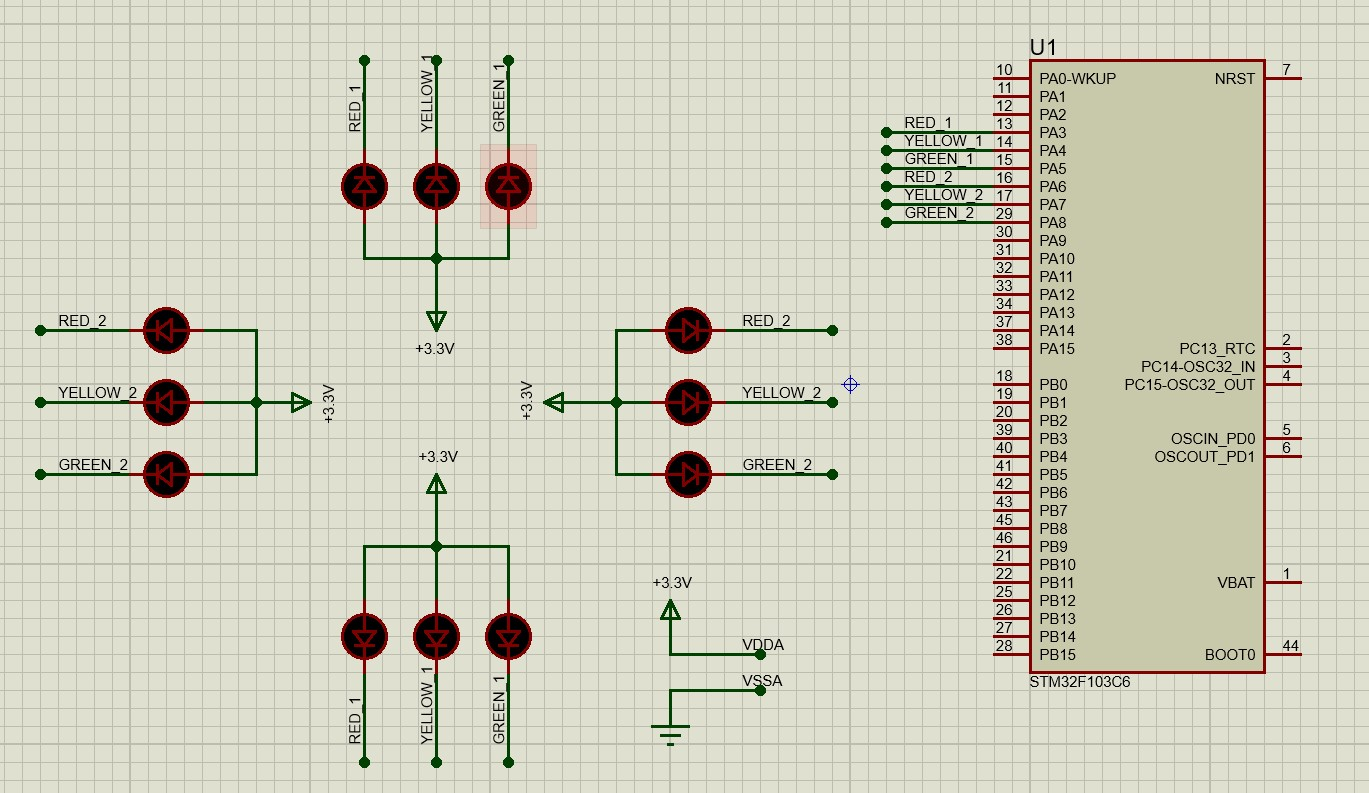
\includegraphics[width=0.8\linewidth]{pictures/schematic_ex03.jpg}
    \caption{\href{https://github.com/Lmonk555/lab01_micro_process_control/tree/147b949f537c459205c0a9d3dc584d4bc5e5fa31/Proteus8/ex_03}{\textit{Proteus schematic for a 4-way traffic light}}}
    \label{schematic_ex03}
\end{figure}

\begin{lstlisting}[language=c,caption={Exercise 03 source code},label={lst:ex03}]
    MX_GPIO_Init();
    /* USER CODE BEGIN 2 */

        GPIO_TypeDef* ledPorts[] = { RED_1_GPIO_Port, YELLOW_1_GPIO_Port, GREEN_1_GPIO_Port,
                                    RED_2_GPIO_Port, YELLOW_2_GPIO_Port, GREEN_2_GPIO_Port };
        uint16_t ledPins[]       = { RED_1_Pin, YELLOW_1_Pin, GREEN_1_Pin,
                                    RED_2_Pin, YELLOW_2_Pin, GREEN_2_Pin };

        //                      	 R1     Y1     G1     R2     Y2     G2
        GPIO_PinState phase1[] = { SET,   SET,   RESET, RESET, SET,   SET   }; // Dir1 green, Dir2 red
        GPIO_PinState phase2[] = { SET,   RESET, SET,   RESET, SET,   SET   }; // Dir1 yellow, Dir2 red
        GPIO_PinState phase3[] = { RESET, SET,   SET,   SET,   SET,   RESET }; // Dir1 red, Dir2 green
        GPIO_PinState phase4[] = { RESET, SET,   SET,   SET,   RESET, SET   }; // Dir1 red, Dir2 yellow

        uint32_t delays[] = { 3000, 2000, 3000, 2000 };
        GPIO_PinState* phases[] = { phase1, phase2, phase3, phase4 };

    /* USER CODE END 2 */

    /* Infinite loop */
    /* USER CODE BEGIN WHILE */
    while (1)
    {
        for (int p = 0; p < 4; p++)
        {
            for (int i = 0; i < 6; i++)
            {
                HAL_GPIO_WritePin(ledPorts[i], ledPins[i], phases[p][i]);
            }
            HAL_Delay(delays[p]);
        }
    }
    /* USER CODE END WHILE */
\end{lstlisting}





\subsection{Exercise 4}
Add \textbf{only one 7 led segment} to the schematic in Exercise 3. This component can be found in Proteus by the keyword \textbf{7SEG-COM-ANODE}. For this device, the common pin should be connected to the power supply and other pins are supposed to connected to PB0 to PB6. Therefore, to turn-on a segment in this 7SEG, the STM32 pin should be in logic 0 (0V).\\

Implement a function named \textbf{display7SEG(int num)}. The input for this function is from 0 to 9 and the outputs are listed as following:

\begin{figure}[!htp]
    \centering
    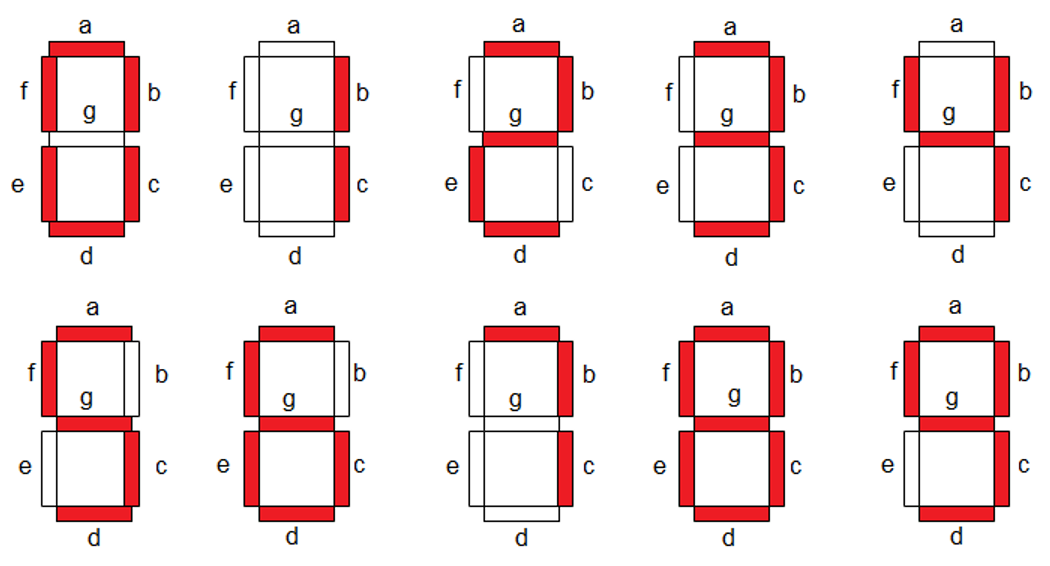
\includegraphics[width=4in]{pictures/bai_1/pic3.PNG}
    \caption{\textit{Display a number on  7 segment LED}}
    \label{bai1_pic3}
\end{figure}

This function is invoked in the while loop for testing as following:
\begin{lstlisting}[caption=An example for your source code]
int counter = 0;
while (1){
    if(counter >= 10) counter = 0;    
    display7SEG(counter++);
    HAL_Delay(1000);

}
\end{lstlisting}

\textbf{Report 1: } Present the schematic.\\

\begin{figure}[H]
    \centering
    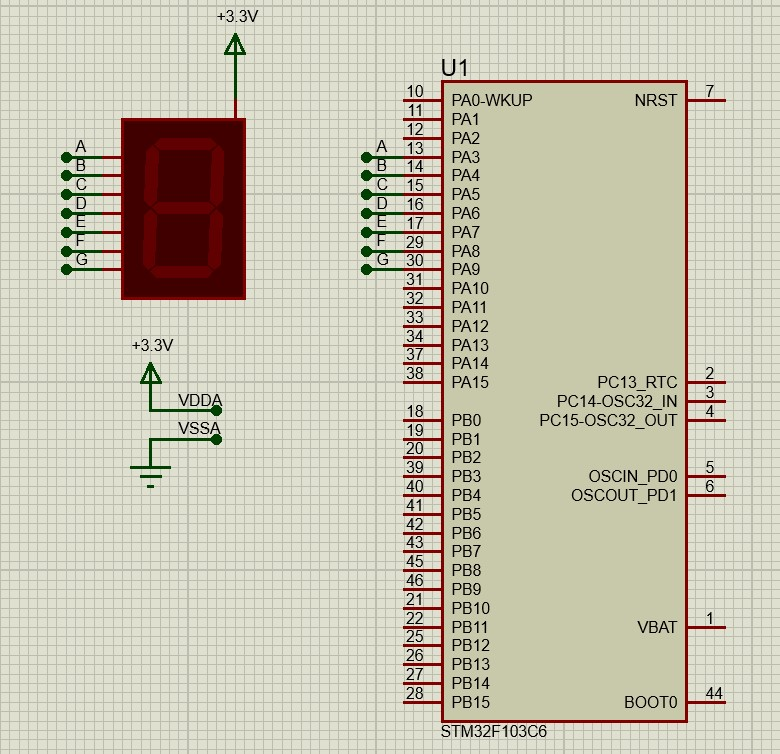
\includegraphics[width=0.8\linewidth]{pictures/schematic_ex04.jpg}
    \caption{\href{https://github.com/Lmonk555/lab01_micro_process_control/tree/d5f2d9541e19f1c1db897d9419e1e3336c01c4b1/Proteus8/ex_04}{\textit{Proteus schematic for a 7-segment LED}}}
    \label{schematic_ex04}
\end{figure}

\textbf{Report 2: } Present the source code for display7SEG function.

\begin{lstlisting}[language=c,caption={Exercise 04 source code},label={lst:ex04}]
    MX_GPIO_Init();
    /* USER CODE BEGIN 2 */

    typedef struct
    {
        GPIO_TypeDef *port;
        uint16_t pin;
    } SegPin;

    SegPin segments[] =
    {
        { A_GPIO_Port, A_Pin },
        { B_GPIO_Port, B_Pin },
        { C_GPIO_Port, C_Pin },
        { D_GPIO_Port, D_Pin },
        { E_GPIO_Port, E_Pin },
        { F_GPIO_Port, F_Pin },
        { G_GPIO_Port, G_Pin },
    };

    GPIO_PinState digitPatterns[10][7] =
    {
        { RESET, RESET, RESET, RESET, RESET, RESET, SET   },	// 0
        { SET,   RESET, RESET, SET,   SET,   SET,   SET   },	// 1
        { RESET, RESET, SET,   RESET, RESET, SET,   RESET },	// 2
        { RESET, RESET, RESET, RESET, SET,   SET,   RESET },	// 3
        { SET,   RESET, RESET, SET,   SET,   RESET, RESET },	// 4
        { RESET, SET,   RESET, RESET, SET,   RESET, RESET },	// 5
        { RESET, SET,   RESET, RESET, RESET, RESET, RESET },	// 6
        { RESET, RESET, RESET, SET,   SET,   SET,   SET   },	// 7
        { RESET, RESET, RESET, RESET, RESET, RESET, RESET },	// 8
        { RESET, RESET, RESET, RESET, SET,   RESET, RESET },	// 9
    };

    void display7SEG(int num)
    {
        for (int i = 0; i < 7; i++)
        {
            HAL_GPIO_WritePin(segments[i].port, segments[i].pin, digitPatterns[num][i]);
        }
    }

    int counter = 0;

    /* USER CODE END 2 */

    /* Infinite loop */
    /* USER CODE BEGIN WHILE */
    while (1)
    {
        if(counter >= 10) counter = 0;
        display7SEG(counter++);
        HAL_Delay(1000);
    }
    /* USER CODE END WHILE */
\end{lstlisting}





\subsection{Exercise 5}
Integrate the 7SEG-LED to the 4 way traffic light. In this case, the 7SEG-LED is used to display countdown value.\\

In this exercise, only source code is required to present. The function display7SEG in previous exercise can be re-used.

\textbf{Report: }\\

\begin{figure}[H]
    \centering
    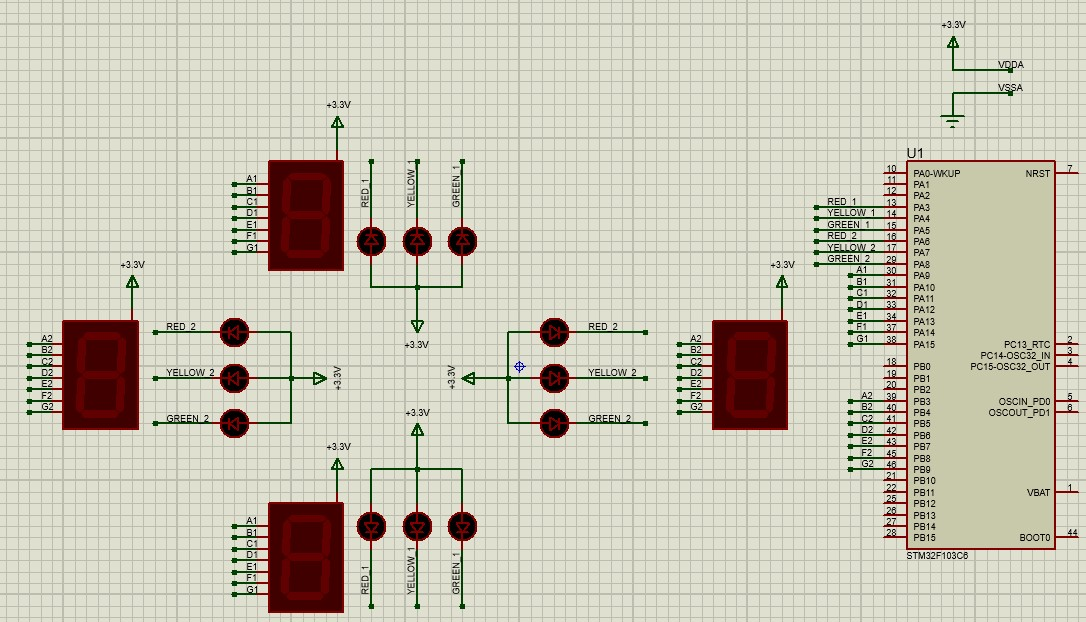
\includegraphics[width=0.8\linewidth]{pictures/schematic_ex05.jpg}
    \caption{\href{https://github.com/Lmonk555/lab01_micro_process_control/tree/d7b362fc0ccbcba37e4b96ebc4d594d433272770/Proteus8/ex_05}{\textit{Proteus schematic for a 4-way traffic with 7-segment LED counters}}}
    \label{schematic_ex05}
\end{figure}

\begin{lstlisting}[language=c,caption={Exercise 05 source code},label={lst:ex05}]
MX_GPIO_Init();
/* USER CODE BEGIN 2 */

    GPIO_TypeDef* ledPorts[] = { RED_1_GPIO_Port, YELLOW_1_GPIO_Port, GREEN_1_GPIO_Port,
                                RED_2_GPIO_Port, YELLOW_2_GPIO_Port, GREEN_2_GPIO_Port };
    uint16_t ledPins[]       = { RED_1_Pin, YELLOW_1_Pin, GREEN_1_Pin,
                                RED_2_Pin, YELLOW_2_Pin, GREEN_2_Pin };

    //                      	 R1     Y1     G1     R2     Y2     G2
    GPIO_PinState phase1[] = { SET,   SET,   RESET, RESET, SET,   SET   }; // GREEN_1, RED_2
    GPIO_PinState phase2[] = { SET,   RESET, SET,   RESET, SET,   SET   }; // YELLOW_1, RED_2
    GPIO_PinState phase3[] = { RESET, SET,   SET,   SET,   SET,   RESET }; // RED_1, GREEN_2
    GPIO_PinState phase4[] = { RESET, SET,   SET,   SET,   RESET, SET   }; // RED_1, YELLOW_2

    void setLeds(GPIO_PinState *pattern)
    {
        for (int i = 0; i < 6; i++)
            HAL_GPIO_WritePin(ledPorts[i], ledPins[i], pattern[i]);
    }

    //##########################################################################################################
    //##########################################################################################################
    //##########################################################################################################

    typedef struct
    {
        GPIO_TypeDef *port;
        uint16_t pin;
    } SegPin;

    SegPin segments_1[] =
    {
        { A1_GPIO_Port, A1_Pin },
        { B1_GPIO_Port, B1_Pin },
        { C1_GPIO_Port, C1_Pin },
        { D1_GPIO_Port, D1_Pin },
        { E1_GPIO_Port, E1_Pin },
        { F1_GPIO_Port, F1_Pin },
        { G1_GPIO_Port, G1_Pin },
    };

    SegPin segments_2[] =
    {
        { A2_GPIO_Port, A2_Pin },
        { B2_GPIO_Port, B2_Pin },
        { C2_GPIO_Port, C2_Pin },
        { D2_GPIO_Port, D2_Pin },
        { E2_GPIO_Port, E2_Pin },
        { F2_GPIO_Port, F2_Pin },
        { G2_GPIO_Port, G2_Pin },
    };

    GPIO_PinState digitPatterns[10][7] =
    {
        { RESET, RESET, RESET, RESET, RESET, RESET, SET   },	// 0
        { SET,   RESET, RESET, SET,   SET,   SET,   SET   },	// 1
        { RESET, RESET, SET,   RESET, RESET, SET,   RESET },	// 2
        { RESET, RESET, RESET, RESET, SET,   SET,   RESET },	// 3
        { SET,   RESET, RESET, SET,   SET,   RESET, RESET },	// 4
        { RESET, SET,   RESET, RESET, SET,   RESET, RESET },	// 5
        { RESET, SET,   RESET, RESET, RESET, RESET, RESET },	// 6
        { RESET, RESET, RESET, SET,   SET,   SET,   SET   },	// 7
        { RESET, RESET, RESET, RESET, RESET, RESET, RESET },	// 8
        { RESET, RESET, RESET, RESET, SET,   RESET, RESET },	// 9
    };

    void display7SEG(SegPin *segs, int num)
    {
        if (num < 0 || num > 9) return;
        for (int i = 0; i < 7; i++)
            HAL_GPIO_WritePin(segs[i].port, segs[i].pin, digitPatterns[num][i]);
    }

    int counter_red = 0;

/* USER CODE END 2 */

/* Infinite loop */
/* USER CODE BEGIN WHILE */
    while (1)
    {
        counter_red = 5;
        setLeds(phase1);						// GREEN 1, RED 2
        for (int i = 3; i >= 1; i--)
        {
            display7SEG(segments_1, i);
            display7SEG(segments_2, counter_red--);
            HAL_Delay(1000);
        }

        setLeds(phase2);						// YELLOW 1, RED 2
        for (int i = 2; i >= 1; i--)
        {
            display7SEG(segments_1, i);
            display7SEG(segments_2, counter_red--);
            HAL_Delay(1000);
        }

        counter_red = 5;
        setLeds(phase3);						// RED 1, GREEN 2
        for (int i = 3; i >= 1; i--)
        {
            display7SEG(segments_2, i);
            display7SEG(segments_1, counter_red--);
            HAL_Delay(1000);
        }

        setLeds(phase4);						// RED 1, GREEN 2
        for (int i = 2; i >= 1; i--)
        {
            display7SEG(segments_2, i);
            display7SEG(segments_1, counter_red--);
            HAL_Delay(1000);
        }
    }
\end{lstlisting}






\subsection{Exercise 6}
In this exercise, a new Proteus schematic is designed to simulate an analog clock, with 12 different number. The connections for 12 LEDs are supposed from PA4 to PA15 of the STM32. The arrangement of 12 LEDs is depicted as follows.

\begin{figure}[H]
    \centering
    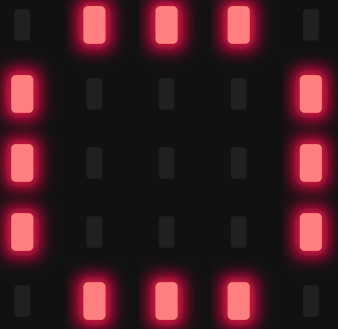
\includegraphics[width=3in]{pictures/bai_1/pic4.PNG}
    \caption{\textit{12 LEDs for an analog clock}}
    \label{bai1_pic3a}
\end{figure}

Report 1: Present the schematic.

\textbf{\textit{*Note: this schematic will be used for Exercise 6-10, along with its code structure.}}

\begin{figure}[H]
    \centering
    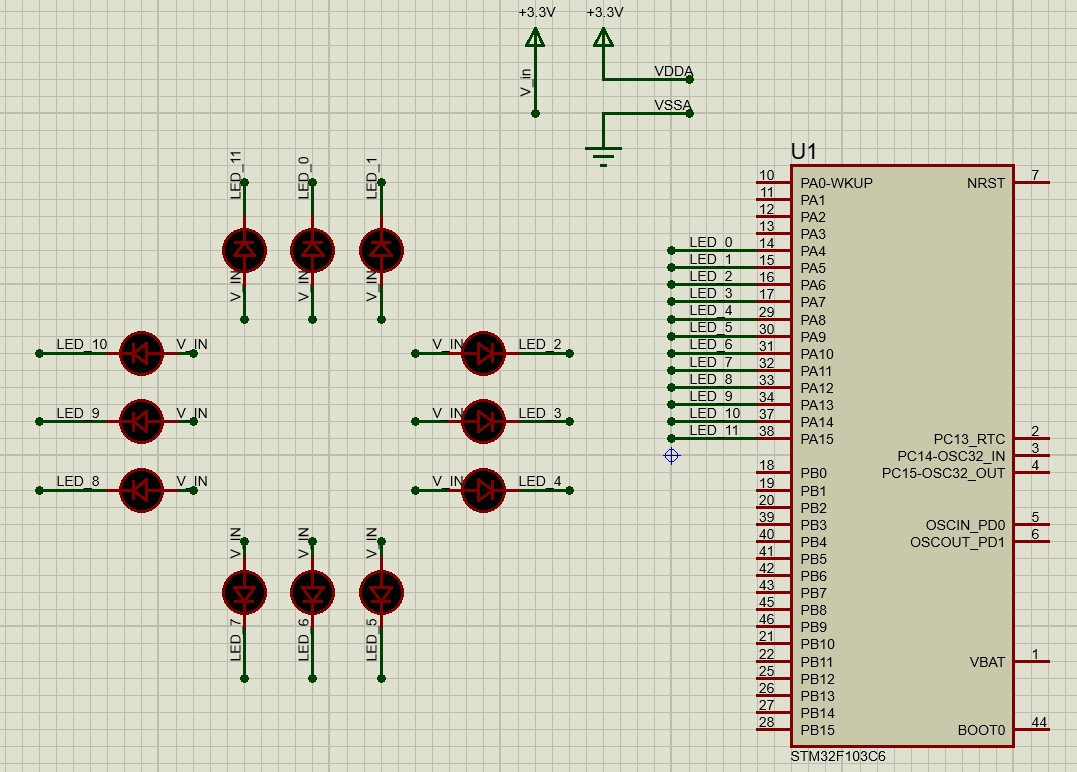
\includegraphics[width=0.8\linewidth]{pictures/schematic_ex_06_to_10.jpg}
    \caption{\href{https://github.com/Lmonk555/lab01_micro_process_control/tree/92474fc35827518ac2bd36b09717d3f81dccfef8/Proteus8/ex_06}{\textit{Proteus schematic for clock by using 12 red LEDs}}}
    \label{schematic_ex06}
\end{figure}

Report 2: Implement a simple program to test the connection of every single LED. This testing program should turn every LED in a sequence.

\begin{lstlisting}[language=c,caption={Exercise 06 source code},label={lst:ex06}]
MX_GPIO_Init();
/* USER CODE BEGIN 2 */

typedef struct
{
    GPIO_TypeDef *port;
    uint16_t pin;
} LedPin;

LedPin clock[] =
{
    { LED_0_GPIO_Port, LED_0_Pin },
    { LED_1_GPIO_Port, LED_1_Pin },
    { LED_2_GPIO_Port, LED_2_Pin },
    { LED_3_GPIO_Port, LED_3_Pin },
    { LED_4_GPIO_Port, LED_4_Pin },
    { LED_5_GPIO_Port, LED_5_Pin },
    { LED_6_GPIO_Port, LED_6_Pin },
    { LED_7_GPIO_Port, LED_7_Pin },
    { LED_8_GPIO_Port, LED_8_Pin },
    { LED_9_GPIO_Port, LED_9_Pin },
    { LED_10_GPIO_Port, LED_10_Pin },
    { LED_11_GPIO_Port, LED_11_Pin },
};

GPIO_PinState state[12][12] =
{
    {RESET, SET, SET, SET, SET, SET, SET, SET, SET, SET, SET, SET},	// 0 & 12
    {SET, RESET, SET, SET, SET, SET, SET, SET, SET, SET, SET, SET},	// 1
    {SET, SET, RESET, SET, SET, SET, SET, SET, SET, SET, SET, SET}, // 2
    {SET, SET, SET, RESET, SET, SET, SET, SET, SET, SET, SET, SET},	// 3
    {SET, SET, SET, SET, RESET, SET, SET, SET, SET, SET, SET, SET},	// 4
    {SET, SET, SET, SET, SET, RESET, SET, SET, SET, SET, SET, SET},	// 5
    {SET, SET, SET, SET, SET, SET, RESET, SET, SET, SET, SET, SET},	// 6
    {SET, SET, SET, SET, SET, SET, SET, RESET, SET, SET, SET, SET},	// 7
    {SET, SET, SET, SET, SET, SET, SET, SET, RESET, SET, SET, SET},	// 8
    {SET, SET, SET, SET, SET, SET, SET, SET, SET, RESET, SET, SET},	// 9
    {SET, SET, SET, SET, SET, SET, SET, SET, SET, SET, RESET, SET},	// 10
    {SET, SET, SET, SET, SET, SET, SET, SET, SET, SET, SET, RESET},	// 11
};

void clearAllClock()
{
    for (int i = 0; i < 12; i++)
        HAL_GPIO_WritePin(clock[i].port, clock[i].pin, SET);
}



/* USER CODE END 2 */

/* Infinite loop */
/* USER CODE BEGIN WHILE */
while (1)
{
    for (int i = 0; i < 12; i++)
    {
        for (int j = 0; j < 12; j++)
            HAL_GPIO_WritePin(clock[j].port, clock[j].pin, state[i][j]);
        HAL_Delay(1000);
    }
}
\end{lstlisting}





\subsection{Exercise 7}
Implement a function named \textbf{clearAllClock()} to turn off all 12 LEDs. Present the source code of this function.

\begin{lstlisting}[caption=Function Implementation]
void clearAllClock(){
    for (int i = 0; i < 12; i++)
        HAL_GPIO_WritePin(clock[i].port, clock[i].pin, SET);
}
\end{lstlisting}





\subsection{Exercise 8}
Implement a function named \textbf{setNumberOnClock(int num)}. The input for this function is from \textbf{0 to 11} and an appropriate LED is turn on. Present the source code of this function.

\begin{lstlisting}[language=c,caption={Exercise 08 source code},label={lst:ex08}]
void setNumberOnClock(int num)
{
    HAL_GPIO_WritePin(clock[num].port, clock[num].pin, GPIO_PIN_RESET);
}
\end{lstlisting}





\subsection{Exercise 9}
Implement a function named \textbf{clearNumberOnClock(int num)}. The input for this function is from \textbf{0 to 11} and an appropriate LED is turn off. 

\begin{lstlisting}[language=c,caption={Exercise 09 source code},label={lst:ex09}]
void clearNumberOnClock(int num)
{
    HAL_GPIO_WritePin(clock[num].port, clock[num].pin, SET);
}
\end{lstlisting}





\subsection{Exercise 10}
Integrate the whole system and use 12 LEDs to display a clock. At a given time, there are only 3 LEDs are turn on for hour, minute and second information.

\begin{lstlisting}[language=c,caption={Exercise 10 source code},label={lst:ex10}]
MX_GPIO_Init();
/* USER CODE BEGIN 2 */

typedef struct
{
    GPIO_TypeDef *port;
    uint16_t pin;
} LedPin;

LedPin clock[] =
{
    { LED_0_GPIO_Port, LED_0_Pin },
    { LED_1_GPIO_Port, LED_1_Pin },
    { LED_2_GPIO_Port, LED_2_Pin },
    { LED_3_GPIO_Port, LED_3_Pin },
    { LED_4_GPIO_Port, LED_4_Pin },
    { LED_5_GPIO_Port, LED_5_Pin },
    { LED_6_GPIO_Port, LED_6_Pin },
    { LED_7_GPIO_Port, LED_7_Pin },
    { LED_8_GPIO_Port, LED_8_Pin },
    { LED_9_GPIO_Port, LED_9_Pin },
    { LED_10_GPIO_Port, LED_10_Pin },
    { LED_11_GPIO_Port, LED_11_Pin },
};

void clearAllClock()
{
    for (int i = 0; i < 12; i++)
        HAL_GPIO_WritePin(clock[i].port, clock[i].pin, GPIO_PIN_SET);
}

void setNumberOnClock(int num)
{
    HAL_GPIO_WritePin(clock[num].port, clock[num].pin, GPIO_PIN_RESET);
}

void clearNumberOnClock(int num)
{
    HAL_GPIO_WritePin(clock[num].port, clock[num].pin, GPIO_PIN_SET);
}

int hour   = 6;
int minute = 49;
int second = 50;

int prevHourPin	= hour % 12;
int prevMinPin	= minute / 5;
int prevSecPin	= second / 5;

clearAllClock();

/* USER CODE END 2 */

/* Infinite loop */
/* USER CODE BEGIN WHILE */
while (1)
{
int hourPin = hour % 12;        // 0-11 directly
int minPin  = minute / 5;       // 0-59 -> 0-11 (each LED = 5 min)
int secPin  = second / 5;       // 0-59 -> 0-11 (each LED = 5 sec)

// Turn off previous clock pin (if different between [now] & [prev])
if (second == 0 || prevHourPin != hourPin) clearNumberOnClock(prevHourPin);
if (second == 0 || prevMinPin  != minPin)  clearNumberOnClock(prevMinPin);
clearNumberOnClock(prevSecPin);

// Change clock pin to current time
setNumberOnClock(hourPin);
setNumberOnClock(minPin);
setNumberOnClock(secPin);

prevHourPin = hourPin;
prevMinPin  = minPin;
prevSecPin  = secPin;

HAL_Delay(1000);

// Second increment
second++;
if (second >= 60)
{
    second = 0;
    minute++;
    if (minute >= 60)
    {
        minute = 0;
        hour++;
        if (hour >= 12) hour = 0;
    }
}
}
\end{lstlisting}



